\chapter{极限与连续}
\section{极限的有关定义}
\begin{definition}{数列极限}{lim}
数列$\{a_n\}$,若对于$ \forall\varepsilon>0 $,$ \exists N>0 $,当$ n>N $时,有
\begin{align}
    \vert{a_n-A}\vert<\varepsilon
\end{align}
则称数列$\{a_n\}$的极限为$A$(或:收敛于$A$),记作
\begin{align}
    \lim_{n\to \infty} a_n=A 
\end{align}
\end{definition}



\begin{definition}{函数极限-1}{limf1}
函数$f(x)$,若对于$ \forall\varepsilon>0 $,$ \exists \delta>0 $,当$ 0<\vert x-a\vert <\delta $时,有
\begin{align}
    \vert{f(x)-A}\vert<\varepsilon
\end{align}
则称函数$f(x)$的极限为$A$,记作
\begin{align}
    \lim_{x\to a} f(x)=A 
\end{align}
\end{definition}

\begin{note}
\begin{enumerate}
    \item 若$x \to a$,则$x\neq a$.如:$ \lim\limits_{x\to 0}\displaystyle\frac{0}{x^3}=0 $;
    \item $\lim\limits_{x \to a}f(x)$ 与$ f(a) $ 无关。如:$\lim\limits_{x \to 1}\displaystyle\frac{x^2-1}{x-1}=\lim\limits_{x \to 1}(x+1)=2$;
    \item $x \to a$分为$ x \to a^{+} $和$ x \to a^{-}$;
    \item 我们称$0<\vert x-a\vert <\delta$为$ a $的去心邻域;
    \item $\lim\limits_{x \to a^-}\triangleq f(a-0)$(左极限);
    $\lim\limits_{x \to a^+}\triangleq f(a+0)$(右极限)。
\end{enumerate}
\end{note}

\FiveStar $\lim\limits_{x \to a} f(x)$存在$\iff f(a-0),f(a+0)$都存在且相等。

\begin{definition}{函数极限-2}{limf2}
函数$f(x)$,若对于$ \forall\varepsilon>0 $,$ \exists X>(<)0 $,当$ x>X(<-X) $时,有
\begin{align}
    \vert{f(x)-A}\vert<\varepsilon
\end{align}
则称函数$f(x)$的极限为$A$,记作
\begin{align}
    \lim_{x\to +\infty(-\infty)} f(x)=A 
\end{align}
\end{definition}

如,对于函数$f(x)=\arctan{x}$有:
 $\lim\limits_{x\to +\infty} f(x)=\displaystyle\frac{\pi}{2}$,$\lim\limits_{x\to -\infty} f(x)=-\displaystyle \frac{\pi}{2}$

 \begin{figure}[htbp]
    \centering
    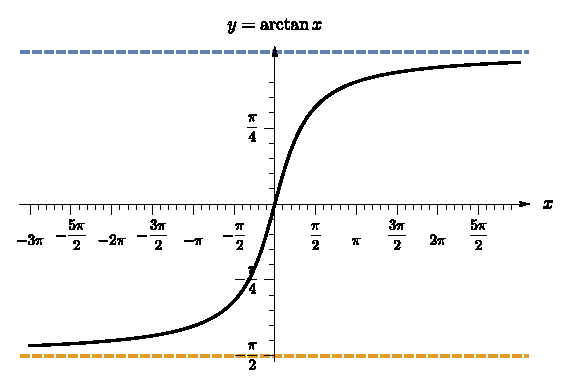
\includegraphics[width=0.7\textwidth]{2.eps}
    \caption{$f(x)=\arctan{x}$的图像}
  \end{figure}
  
\begin{definition}{无穷小}{wqx}
若 $ \lim\limits_{x \to a} \alpha(x)=0$,则称$ \alpha(x)$当$x \to a$时为无穷小。
\end{definition}

\begin{note}
\begin{enumerate}
  \item 0是无穷小,但无穷小不一定为0;
  \item $\alpha(x)\neq 0$,$\alpha(x)$是否为无穷小与$ x $的\CJKunderdot{趋向}有关;如,$\alpha=3(x-1)^2$,而$\lim\limits_{x \to 1}\alpha=0 $,则$3(x-1)^2$当$x \to 1$时是无穷小。
  \item 设$\alpha \to 0,\beta \to 0$,有如下三种情形:
  
  (a) $\lim \displaystyle\frac{\beta}{\alpha}=0$,称$ \beta $为$ \alpha $的高阶无穷小,记作$\beta=o(\alpha)$;
  
  (b) $\lim \displaystyle\frac{\beta}{\alpha}=k(\neq \infty,0)$,称$ \beta $为$ \alpha $的同阶无穷小,记作$\beta=O(\alpha)$(特例:$\lim \displaystyle\frac{\beta}{\alpha}$=1,则称$ \beta $与$ \alpha $为等价无穷小,记作$\beta \sim \alpha$)。
\end{enumerate}
\end{note}


\section{极限的性质}
\subsection{极限的一般性质}
下面我们开始介绍极限的一般性质,并给出相关的证明。主要有:唯一性、保号性(重点)两个性质。
\begin{enumerate}
    \item 唯一性
    \begin{property}
        极限存在必唯一。
    \end{property}
    
    \begin{proof}
    设$\lim\limits_{x \to a}f(x)=A $
    又$ \lim\limits_{x \to a}f(x)=B $,并不妨设$A>B$。我们采用反证法来完成相关的证明。
    
    取$ \varepsilon=\displaystyle\frac{A-B}{2}>0 $。因为$\lim\limits_{x \to a}f(x)=A $,所以存在$\delta_1>0 $,当 $0<\vert x-a\vert <\delta_1 $时,有$\vert{f(x)-A}\vert<\displaystyle\frac{A-B}{2}$,也即$\displaystyle\frac{A+B}{2}<f(x)<\frac{3A-B}{2}(*)$; 
    
    
    同理,由第二个极限可以得出$\displaystyle\frac{3B-A}{2}<f(x)<\displaystyle\frac{A+B}{2}(**)$。从而,若我们取$\delta=\min{(\delta_1,\delta_2)}$,当
    $ 0<\vert x-a\vert <\delta $时,就有$(*)$与$(**)$同时成立。但$f(x)>\displaystyle\frac{A+B}{2}$与$f(x)<\displaystyle\frac{A+B}{2}$显然不可能同时成立,矛盾,从而假设不成立。
    
    同理,我们可以得到$A<B$也不成立。故$A=B$。
    \end{proof}
    
    \item \FiveStar 保号性
    \begin{property}
        设$\lim\limits_{x \to a}f(x)=A>(<)0$,则存在$ \delta>0 $,当$ 0<\vert x-a\vert <\delta $时,有$f(x)>(<)0$。
    \end{property}
    \begin{proof}
        设$A>0$。取$\varepsilon=\displaystyle\frac{1}{2}A>0$。因为$\lim\limits_{x \to a}f(x)=A$,故存在$ \delta>0 $,当$ 0<\vert x-a\vert <\delta $时,有 $\vert{f(x)-A}\vert<\varepsilon=\displaystyle\frac{A}{2}$。展开可得$\displaystyle\frac{A}{2}<f(x)<\displaystyle\frac{3}{2}A$。从而$f(x)>0$。
    \end{proof}
    \begin{example}
       若函数$ f(x) $ 满足$ f(1)=0, \lim\limits_{x \to 1} \displaystyle\frac{f'(x)}{(x-1)^3}=-2 $,则$ x=1 $为什么点?
    \end{example}
    \begin{solution}
        因为$\lim\limits_{x \to 1}\displaystyle\frac{f'(x)}{(x-1)^3}=-2<0$,故根据保号性,存在$ \delta>0 $,当$ 0<\vert x-a\vert <\delta $时,有$\displaystyle\frac{f'(x)}{(x-1)^3}<0$。于是,当$x \in (1-\delta,1)$时,$f'(x)>0$;当$x \in (1,1+\delta)$时,$f'(x)<0$。故$x=1$为极大值点。
    \end{solution}
\end{enumerate}

    \subsection{极限的存在性质}
    下面介绍几个判定极限\textbf{存在}的性质。
    \begin{property}
    \begin{enumerate}
        \item 数列型
       
        如果$ a_n\leq b_n\leq c_n $且$ \lim\limits_{n \to \infty}a_n=\lim\limits_{n \to \infty}c_n=A $,则$ \lim\limits_{n \to \infty}b_n=A $。
        \item 函数型
        
        如果$ f(x)\leq g(x)\leq h(x) $且$ \lim\limits_{x \to a}f(x)=\lim\limits_{x \to a}h(x)=A $,则$ \lim\limits_{x \to a}g(x)=A $。
    \end{enumerate}
    \end{property}
    \subsubsection*{型一例题:$n$项和求极限}
    \begin{example}
        求极限:$\lim\limits_{n \to \infty}(\displaystyle\frac{1}{\sqrt{n^2+1}}+\displaystyle\frac{1}{\sqrt{n^2+2}}+ \cdots +\frac{1}{\sqrt{n^2+n}})$
    \end{example}
    \begin{solution}
        以上是非齐次的情形,采取夹逼定理。于是令$b_n=\displaystyle\frac{1}{\sqrt{n^2+1}}+\displaystyle\frac{1}{\sqrt{n^2+2}}+ \cdots +\frac{1}{\sqrt{n^2+n}}$。
        
        容易得到:
        $\displaystyle\frac{n}{\sqrt{n^2+n}}\leq b_n \leq \displaystyle\frac{n}{\sqrt{n^2+1}}$,
        
        因为$\lim\limits_{n \to \infty}\displaystyle\frac{n}{\sqrt{n^2+n}}=\lim\limits_{n\to\infty}\displaystyle\frac{1}{\sqrt{\frac{1}{n}+1}}=1$且$\lim\limits_{n \to \infty}\displaystyle\frac{n}{\sqrt{n^2+1}}=\lim\limits_{n\to\infty}\displaystyle\frac{1}{\sqrt{\frac{1}{n^2}+1}}=1$,故得到$\lim\limits_{n \to \infty}b_n=1$。
    \end{solution}

    \begin{example}
        求极限$ \lim\limits_{n \to \infty}(\displaystyle\frac{1}{n^2+1}+\displaystyle\frac{1}{n^2+2}+\cdots+\displaystyle\frac{n}{n^2+n}) $。
    \end{example}
    \begin{solution}
        令$ b_n=\displaystyle\frac{1}{n^2+1}+\displaystyle\frac{1}{n^2+2}+\cdots+\displaystyle\frac{n}{n^2+n}$,从而$\displaystyle\frac{1}{2}=\displaystyle\frac{n(n+1)}{2(n^2+n)} \leq b_n \leq\displaystyle\frac{n(n+1)}{2(n^2+1)}$。则$\lim\limits_{n \to \infty}$左$=\lim\limits_{n \to \infty}$右$=\displaystyle\frac{1}{2}$。故所求极限为$\displaystyle\frac{1}{2}$。
    \end{solution}

    \begin{example}
        求极限$ \lim\limits_{n \to \infty}(\displaystyle\frac{1}{n+1}+\displaystyle\frac{1}{n+2}+\cdots+\displaystyle\frac{1}{n+n}) $。
    \end{example}
    \begin{solution}
        \begin{align*}
            \lim_{n \to \infty}(\frac{1}{n+1}+\frac{1}{n+2}+\cdots+\frac{1}{n+n})
            &=\lim_{n \to \infty}\sum_{i=1}^n\frac{1}{n+i} \\
            &=\lim_{n \to \infty}\frac{1}{n}\sum_{i=1}^n\frac{n}{n+i}\\
            &=\lim_{n \to \infty}\frac{1}{n}\sum_{i=1}^n\frac{1}{1+\frac{i}{n}}\\
            &= \int_0^1\frac{1}{1+x}\mathrm{d}x=\ln(x+1)\bigg|_{0} ^1=\ln 2
        \end{align*}
    \end{solution}

    \begin{example}
        求极限$ \lim\limits_{n \to \infty}(\displaystyle\frac{n}{n^2+1^2}+\displaystyle\frac{n}{n^2+2^2}+\cdots+\displaystyle\frac{n}{n^2+n^2}) $。
    \end{example}
    \begin{solution}
        \begin{align*}
            \lim_{n \to \infty}(\frac{n}{n^2+1^2}+\frac{n}{n^2+2^2}+\cdots+\frac{n}{n^2+n^2})
            &=\lim_{n \to \infty}\sum_{i=1}^n\frac{n}{n^2+i^2} \\
            &=\lim_{n \to \infty}\frac{1}{n}\sum_{i=1}^n\frac{n^2}{n^2+i^2}\\
            &=\lim_{n \to \infty}\frac{1}{n}\sum_{i=1}^n\frac{1}{1+\frac{i^2}{n^2}}\\
            &= \int_0^1\frac{1}{1+x^2}\mathrm{d}x=\arctan x\bigg|_{0} ^1=\frac{\pi}{4}
        \end{align*}
    \end{solution}
    \begin{note}
        对于$n$个数相加,分子或分母不齐次的情况,用夹逼定理;
        
        对于分子、分母齐次且分母多一次的情况,用定积分定义。
    \end{note}
    我们还有另一个著名的判定数列极限存在性的定理,也即如下性质:
    \begin{property}
        单调有界数列必有极限。
    \end{property}
    这个性质可以分为两类来讨论,一为单调递增有上界,二为单调递减有下界。
    \subsubsection*{型二例题:极限存在性证明}
    \begin{example}
        已知,$a_1=\sqrt{2}, a_2=\sqrt{2+\sqrt{2}}, a_3=\sqrt{2+\sqrt{2+\sqrt{2}}}, \cdots$

        证明$\lim\limits_{n \to \infty}a_n$存在,并求之。
    \end{example}
    \begin{solution}
        显然,$ \{a_n\} $单调递增,现在我们证明$ a_n \leq 2$,采用数学归纳法:

        首先,$ a_1=\sqrt{2}<2 $。假设$a_k\leq 2$,则$a_{k+1} =\sqrt{2+a_k}\leq \sqrt{2+2}=2$。因此 $a_n \leq 2$。从而由单调有界定理知$\lim\limits_{n \to \infty}a_n$存在。下面求出这个极限:

        设极限为$A$,由$a_{n+1}=\sqrt{2+a_n}$,令$ n \to \infty $,两边平方有$ A^2=A+2 $,解得$ A=2 $或 $ A=-1 $。由于$a_n>a_1=\sqrt{2}$,故$ A=-1 $舍去。从而极限为$ 2 $。
    \end{solution}

    \begin{example}
        已知$ a_1=2, a_{n+1}=\displaystyle\frac{1}{2}(a_n+\displaystyle\frac{1}{a_n})$。证明:$\lim\limits_{n \to \infty}a_n$存在。
    \end{example}
    \begin{solution}
        先证明$ a_n>0 $:
        由于$a_1>0$,故设$a_k>0$。则$a_{k+1}=\displaystyle\frac{1}{2}(a_k+\displaystyle\frac{1}{a_{k+1}})>0$。于是根据均值不等式可以得到$a_{n+1} \geq 1$。而$a_{n+1}-a_n=\displaystyle\frac{1}{2}(a_n+\displaystyle\frac{1}{a_{n+1}})-a_n=\displaystyle\frac{1}{2}(\displaystyle\frac{1}{a_n}-a_{n+1})$。由于$a_{n} \geq 1$,故$\displaystyle\frac{1}{a_n} \leq a_n$。从而,$a_{n+1}-a_n \leq 0$。于是数列$ \{a_n\} $单调递减,又有$a_n \geq 1$,从而得到$\lim\limits_{n \to \infty}a_n$存在。
    \end{solution}

    \subsection{无穷小的性质}
    \subsubsection*{(一)一般性质}
    \begin{enumerate}
        \item 若$ \alpha \to 0 $且$ \beta \to 0 $,则:
        \[ \left\{
            \begin{array}{rl}
                & \alpha \pm \beta  \to 0,\\
                & k \alpha  \to 0,\\
                & \alpha \beta  \to 0.
            \end{array} \right. \]
        \item 若$ \vert \alpha \vert \leq M, \beta \to 0$,则$\alpha \beta \to 0$。
        \item $\alpha \to 0, \lim\limits f(x)=A \Leftrightarrow f(x)=A+\alpha$。
    \end{enumerate}
    \subsubsection*{(二)等价性质}
    \begin{enumerate}
        \item \begin{enumerate}
            \item $ \alpha \sim \alpha $(自反性);
            \item $ \alpha \sim \beta \Rightarrow \beta \sim \alpha $(对称性);
            \item $ \alpha \sim \beta , \beta \sim \gamma \Rightarrow \alpha \sim \gamma $(传递性)。
        \end{enumerate}
        \item $ \alpha \sim \alpha_1, \beta \sim \beta_1, \lim \displaystyle\frac{\beta_1}{\alpha_1} =A$,则$\lim \displaystyle\frac{\beta}{\alpha} =A$。
        \item \textbf{当$x \to 0$时:} \begin{enumerate}
            \item $x \sim \sin x \sim \tan x \sim \arcsin x \sim \arctan x \sim \mathrm{e}^x -1 \sim \ln{(x+1)}$;
            \item $1- \cos x \sim \displaystyle\frac{1}{2} x^2$;
            \item $(1+x)^a-1 \sim ax$。
        \end{enumerate}
    \end{enumerate}
    
    \section{两个重要极限}
    \subsection{准备工作}
    我们先证明如下结论:

    当$ 0<x<\displaystyle\frac{\pi}{2} $时,有
    \begin{align*}
        \sin x<x<\tan x
    \end{align*}
        \begin{proof}
        如图\ref{dwy}所示,在单位圆中,当$ 0<x<\displaystyle\frac{\pi}{2}$时,有
        $S_{\bigtriangleup AOB}=\displaystyle\frac{1}{2}r^2 \sin x=\displaystyle\frac{1}{2}\sin x=S_1$, 
        $S_{\text{扇形} AOB}=\displaystyle\frac{1}{2}x=S_2$, 
        $S_{\mathrm{Rt} \bigtriangleup AOC}=\displaystyle\frac{1}{2}AC=\displaystyle\frac{1}{2}\tan x=S_3$。
        
        显然有
        \begin{align*}
            S_3>S_2>S_1
        \end{align*}
        从而,
        \begin{align*}
            \frac{1}{2}\tan x>\frac{1}{2}x>\frac{1}{2}\sin x
        \end{align*}
        于是,$\sin x<x<\tan x$证明完毕。
        \begin{figure}[htbp]
            \centering
            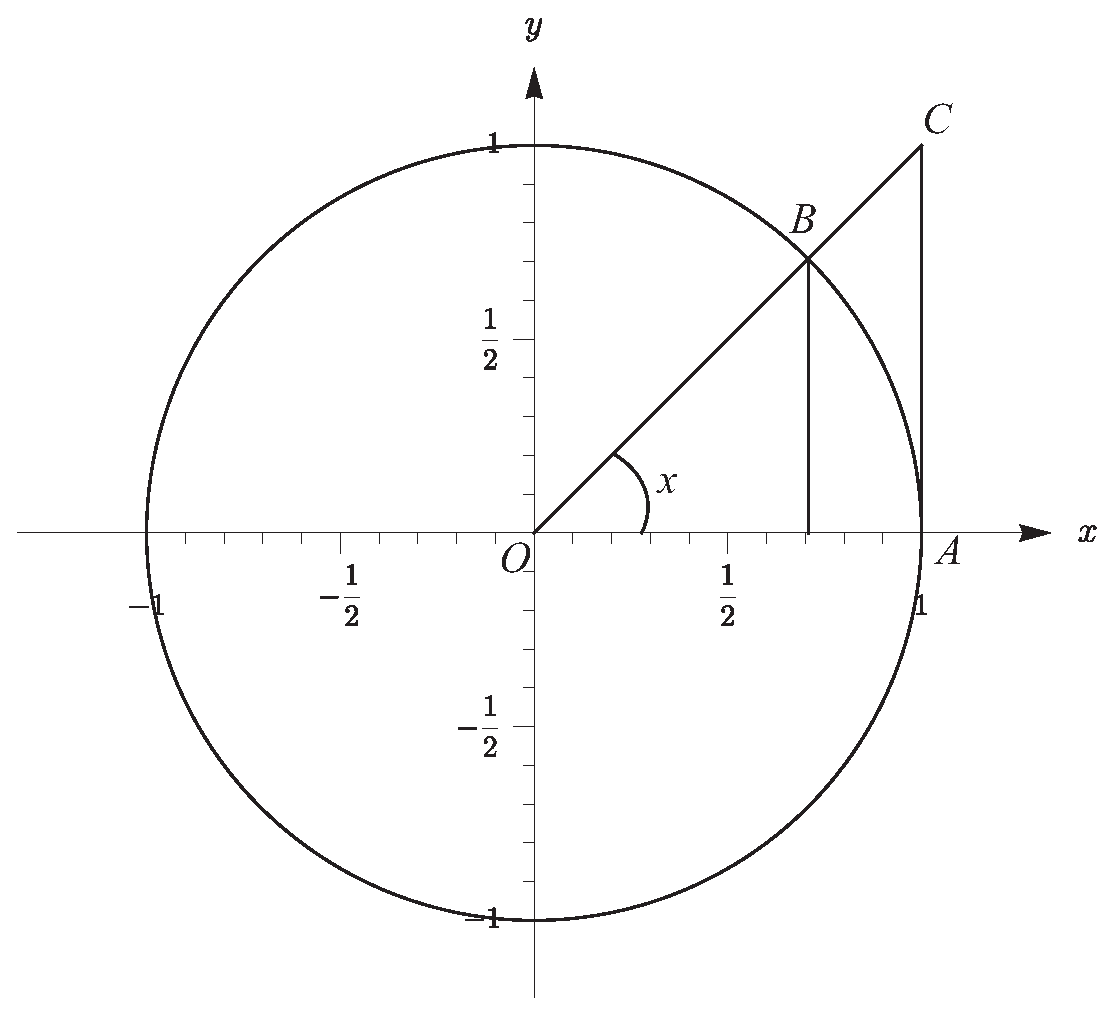
\includegraphics[width=0.7\textwidth]{3.eps}
            \caption{单位圆}
            \label{dwy}
          \end{figure}
        \end{proof}
        \begin{note}
            这里给出的证明并不够严谨,但更严密的证明需要引入幂级数对$\sin x$进行重新定义,这里不再阐述。
        \end{note}
        
        \subsection{两个重要极限式}
        \begin{enumerate}
            \item $\lim\limits_{\Delta \to 0} \frac{\sin \Delta}{\Delta}=1$
            \item $\lim\limits_{\Delta \to 0} (1+\Delta)^{\frac{1}{\Delta}}=\mathrm{e}$
        \end{enumerate}
        \begin{note}
            这里的$\Delta$表示一切具有趋于零状态的变量与表达式,需要当作一个整体来进行处理。
        \end{note}

        \subsubsection*{型三例题:不定型}
        所谓不定型,就是指含有“无穷”与0的极限求解。包含$ 
        \frac{0}{0} $型,$ 1^{\infty} $型,$ 
        \frac{\infty}{\infty} $型,$ 
        \infty \times \infty $型,$ 
        \infty - \infty $型,$ 
        \infty^{0} $型与$0^{0} $型。

        下面分类进行讲解。
        \begin{enumerate}
            \item $ \displaystyle\frac{0}{0} $型
            
            \begin{enumerate}
                \item 习惯:    
                    \[ \left\{
                        \begin{array}{rl}
                            & u(x)^{v(x)}  \Rightarrow \mathrm{e}^{v(x)\ln u(x)},\\
                            & \ln {(\quad )}   \Rightarrow \ln{(1+\Delta)} \sim \Delta(\Delta \to 0),\\
                            & (\quad)-1  \Rightarrow \left\{ \begin{array}{rl} & \mathrm{e}^{\Delta}-1  \sim \Delta;\\
                                & (1+\Delta)^a-1  \sim a\Delta.
                            \end{array} \right. (\Delta \to 0)\\
                            & x-\ln (1+x) \Rightarrow \text{二阶无穷小},\\
                            & x,\sin x,\tan x, \arcsin x, \arctan x \Rightarrow \text{任意两个之差为三阶无穷小}。
                        \end{array} \right. \]
                \item 注意:例如,$\lim\limits_{x \to 0} \displaystyle\frac{x-\sin x}{x^3} \neq \lim\limits_{x \to 0} \displaystyle\frac{x-x}{x^3}=0$
            \end{enumerate}

            \begin{example}
              求极限: $ \lim\limits_{x\to 0} \displaystyle\frac{\tan x-\sin x}{x^3}$。
            \end{example}
            
            \begin{solution}
                \begin{align*}
                   \text{原式}
                   &=\lim_{x \to 0}\frac{\tan(1-\cos x)}{x^3}\\
                    &=\lim_{x \to 0}\frac{x(\frac{1}{2}x^2)}{x^3}=\frac{1}{2}
                \end{align*}
                     
            \end{solution}
        \end{enumerate}



   